\PassOptionsToPackage{unicode=true}{hyperref} % options for packages loaded elsewhere
\PassOptionsToPackage{hyphens}{url}
%
\documentclass[]{book}
\usepackage{lmodern}
\usepackage{amssymb,amsmath}
\usepackage{ifxetex,ifluatex}
\usepackage{fixltx2e} % provides \textsubscript
\ifnum 0\ifxetex 1\fi\ifluatex 1\fi=0 % if pdftex
  \usepackage[T1]{fontenc}
  \usepackage[utf8]{inputenc}
  \usepackage{textcomp} % provides euro and other symbols
\else % if luatex or xelatex
  \usepackage{unicode-math}
  \defaultfontfeatures{Ligatures=TeX,Scale=MatchLowercase}
\fi
% use upquote if available, for straight quotes in verbatim environments
\IfFileExists{upquote.sty}{\usepackage{upquote}}{}
% use microtype if available
\IfFileExists{microtype.sty}{%
\usepackage[]{microtype}
\UseMicrotypeSet[protrusion]{basicmath} % disable protrusion for tt fonts
}{}
\IfFileExists{parskip.sty}{%
\usepackage{parskip}
}{% else
\setlength{\parindent}{0pt}
\setlength{\parskip}{6pt plus 2pt minus 1pt}
}
\usepackage{hyperref}
\hypersetup{
            pdftitle={Environmental Systems Data Science},
            pdfauthor={Loïc Pellissier, Joshua Payne, Benjamin Stocker},
            pdfborder={0 0 0},
            breaklinks=true}
\urlstyle{same}  % don't use monospace font for urls
\usepackage{color}
\usepackage{fancyvrb}
\newcommand{\VerbBar}{|}
\newcommand{\VERB}{\Verb[commandchars=\\\{\}]}
\DefineVerbatimEnvironment{Highlighting}{Verbatim}{commandchars=\\\{\}}
% Add ',fontsize=\small' for more characters per line
\usepackage{framed}
\definecolor{shadecolor}{RGB}{248,248,248}
\newenvironment{Shaded}{\begin{snugshade}}{\end{snugshade}}
\newcommand{\AlertTok}[1]{\textcolor[rgb]{0.94,0.16,0.16}{#1}}
\newcommand{\AnnotationTok}[1]{\textcolor[rgb]{0.56,0.35,0.01}{\textbf{\textit{#1}}}}
\newcommand{\AttributeTok}[1]{\textcolor[rgb]{0.77,0.63,0.00}{#1}}
\newcommand{\BaseNTok}[1]{\textcolor[rgb]{0.00,0.00,0.81}{#1}}
\newcommand{\BuiltInTok}[1]{#1}
\newcommand{\CharTok}[1]{\textcolor[rgb]{0.31,0.60,0.02}{#1}}
\newcommand{\CommentTok}[1]{\textcolor[rgb]{0.56,0.35,0.01}{\textit{#1}}}
\newcommand{\CommentVarTok}[1]{\textcolor[rgb]{0.56,0.35,0.01}{\textbf{\textit{#1}}}}
\newcommand{\ConstantTok}[1]{\textcolor[rgb]{0.00,0.00,0.00}{#1}}
\newcommand{\ControlFlowTok}[1]{\textcolor[rgb]{0.13,0.29,0.53}{\textbf{#1}}}
\newcommand{\DataTypeTok}[1]{\textcolor[rgb]{0.13,0.29,0.53}{#1}}
\newcommand{\DecValTok}[1]{\textcolor[rgb]{0.00,0.00,0.81}{#1}}
\newcommand{\DocumentationTok}[1]{\textcolor[rgb]{0.56,0.35,0.01}{\textbf{\textit{#1}}}}
\newcommand{\ErrorTok}[1]{\textcolor[rgb]{0.64,0.00,0.00}{\textbf{#1}}}
\newcommand{\ExtensionTok}[1]{#1}
\newcommand{\FloatTok}[1]{\textcolor[rgb]{0.00,0.00,0.81}{#1}}
\newcommand{\FunctionTok}[1]{\textcolor[rgb]{0.00,0.00,0.00}{#1}}
\newcommand{\ImportTok}[1]{#1}
\newcommand{\InformationTok}[1]{\textcolor[rgb]{0.56,0.35,0.01}{\textbf{\textit{#1}}}}
\newcommand{\KeywordTok}[1]{\textcolor[rgb]{0.13,0.29,0.53}{\textbf{#1}}}
\newcommand{\NormalTok}[1]{#1}
\newcommand{\OperatorTok}[1]{\textcolor[rgb]{0.81,0.36,0.00}{\textbf{#1}}}
\newcommand{\OtherTok}[1]{\textcolor[rgb]{0.56,0.35,0.01}{#1}}
\newcommand{\PreprocessorTok}[1]{\textcolor[rgb]{0.56,0.35,0.01}{\textit{#1}}}
\newcommand{\RegionMarkerTok}[1]{#1}
\newcommand{\SpecialCharTok}[1]{\textcolor[rgb]{0.00,0.00,0.00}{#1}}
\newcommand{\SpecialStringTok}[1]{\textcolor[rgb]{0.31,0.60,0.02}{#1}}
\newcommand{\StringTok}[1]{\textcolor[rgb]{0.31,0.60,0.02}{#1}}
\newcommand{\VariableTok}[1]{\textcolor[rgb]{0.00,0.00,0.00}{#1}}
\newcommand{\VerbatimStringTok}[1]{\textcolor[rgb]{0.31,0.60,0.02}{#1}}
\newcommand{\WarningTok}[1]{\textcolor[rgb]{0.56,0.35,0.01}{\textbf{\textit{#1}}}}
\usepackage{longtable,booktabs}
% Fix footnotes in tables (requires footnote package)
\IfFileExists{footnote.sty}{\usepackage{footnote}\makesavenoteenv{longtable}}{}
\usepackage{graphicx,grffile}
\makeatletter
\def\maxwidth{\ifdim\Gin@nat@width>\linewidth\linewidth\else\Gin@nat@width\fi}
\def\maxheight{\ifdim\Gin@nat@height>\textheight\textheight\else\Gin@nat@height\fi}
\makeatother
% Scale images if necessary, so that they will not overflow the page
% margins by default, and it is still possible to overwrite the defaults
% using explicit options in \includegraphics[width, height, ...]{}
\setkeys{Gin}{width=\maxwidth,height=\maxheight,keepaspectratio}
\setlength{\emergencystretch}{3em}  % prevent overfull lines
\providecommand{\tightlist}{%
  \setlength{\itemsep}{0pt}\setlength{\parskip}{0pt}}
\setcounter{secnumdepth}{5}
% Redefines (sub)paragraphs to behave more like sections
\ifx\paragraph\undefined\else
\let\oldparagraph\paragraph
\renewcommand{\paragraph}[1]{\oldparagraph{#1}\mbox{}}
\fi
\ifx\subparagraph\undefined\else
\let\oldsubparagraph\subparagraph
\renewcommand{\subparagraph}[1]{\oldsubparagraph{#1}\mbox{}}
\fi

% set default figure placement to htbp
\makeatletter
\def\fps@figure{htbp}
\makeatother

\usepackage{booktabs}
\usepackage[]{natbib}
\bibliographystyle{apalike}

\title{Environmental Systems Data Science}
\author{Loïc Pellissier, Joshua Payne, Benjamin Stocker}
\date{2020-06-24}

\begin{document}
\maketitle

{
\setcounter{tocdepth}{1}
\tableofcontents
}
\hypertarget{primers}{%
\chapter{Primers}\label{primers}}

(Youtube videos can be embedded, according to \href{https://bookdown.org/yihui/rmarkdown/learnr-videos.html}{this}, but it didn't work for me.)

\hypertarget{exercises}{%
\section{Exercises}\label{exercises}}

\hypertarget{overview}{%
\subsection{Overview}\label{overview}}

\begin{itemize}
\tightlist
\item
  \textbf{Input}: Reads for the first time the dataset 1 of two (Swiss) FLUXNET sites at high temporal resolution with 3-4 measures.
\item
  \textbf{Output}: Learned about the data structure and the capacity to explore the content of the dataframe and visualize it so that it can be analysed in the next session.
\item
  \textbf{Data}: Dataset 1 First hands-on with one of two (Swiss) FLUXNET sites at high temporal resolution with 3-4 measureswith high-resolution fluxnet dataset
\end{itemize}

\textbf{Contents}

\begin{itemize}
\tightlist
\item
  Content and operations:
\item
  Managing the workspace and data
\item
  Basic operations in R
\item
  RStudio, debugging
\item
  Reading a table into a data frame
\item
  Objects, data frames, lists
\item
  Applying a function, loop, etc.
\item
  Simple plotting
\item
  Making workflow reproducible

  \begin{itemize}
  \tightlist
  \item
    RMarkdown
  \end{itemize}
\item
  Coding

  \begin{itemize}
  \tightlist
  \item
    Best practices
  \item
    Modularity
  \end{itemize}
\item
  Version control with git (for dummies: GitHub, fork, clone, commit, push, pull, branch)
\end{itemize}

\hypertarget{reading-data-into-r}{%
\subsection{Reading data into R}\label{reading-data-into-r}}

Load libraries.

\begin{Shaded}
\begin{Highlighting}[]
\KeywordTok{library}\NormalTok{(readr)}
\KeywordTok{library}\NormalTok{(tidyverse)}
\end{Highlighting}
\end{Shaded}

Read data from Laegern site.

\begin{Shaded}
\begin{Highlighting}[]
\NormalTok{df_fluxes <-}\StringTok{ }\KeywordTok{read_csv}\NormalTok{(}\StringTok{"./data/FLX_CH-Lae_FLUXNET2015_FULLSET_HH_2004-2014_1-3.csv"}\NormalTok{, ) }
\end{Highlighting}
\end{Shaded}

\begin{verbatim}
## Parsed with column specification:
## cols(
##   .default = col_double()
## )
\end{verbatim}

\begin{verbatim}
## See spec(...) for full column specifications.
\end{verbatim}

Plot something.

\begin{Shaded}
\begin{Highlighting}[]
\KeywordTok{ggplot}\NormalTok{(}\DataTypeTok{data =} \KeywordTok{slice}\NormalTok{(df_fluxes, }\DecValTok{1}\OperatorTok{:}\DecValTok{1000}\NormalTok{), }\KeywordTok{aes}\NormalTok{(}\DataTypeTok{x =}\NormalTok{ TIMESTAMP_START, NEE_VUT_REF)) }\OperatorTok{+}
\StringTok{  }\KeywordTok{geom_line}\NormalTok{()}
\end{Highlighting}
\end{Shaded}

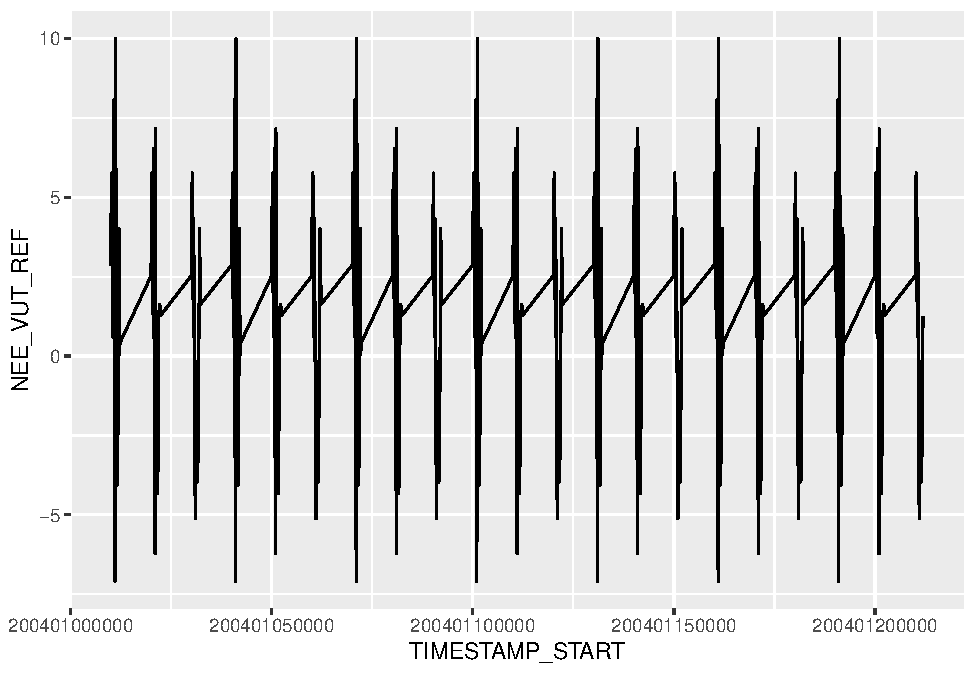
\includegraphics{esds_files/figure-latex/unnamed-chunk-4-1.pdf}

\hypertarget{how-to-use-bookdown-and-markdown}{%
\section{How to use Bookdown and Markdown}\label{how-to-use-bookdown-and-markdown}}

This is a \emph{sample} book written in \textbf{Markdown}. You can use anything that Pandoc's Markdown supports, e.g., a math equation \(a^2 + b^2 = c^2\).

The \textbf{bookdown} package can be installed from CRAN or Github:
nothing

\begin{Shaded}
\begin{Highlighting}[]
\KeywordTok{install.packages}\NormalTok{(}\StringTok{"bookdown"}\NormalTok{)}
\CommentTok{# or the development version}
\CommentTok{# devtools::install_github("rstudio/bookdown")}
\end{Highlighting}
\end{Shaded}

If you want to generate PDF output, you will need to install LaTeX. For R Markdown users who have not installed LaTeX before, we recommend that you install TinyTeX (\url{https://yihui.name/tinytex/}):

\begin{Shaded}
\begin{Highlighting}[]
\KeywordTok{install.packages}\NormalTok{(}\StringTok{'tinytex'}\NormalTok{)}
\NormalTok{tinytex}\OperatorTok{::}\KeywordTok{install_tinytex}\NormalTok{()  }\CommentTok{# install TinyTeX}
\NormalTok{Remember each Rmd file contains one and only one chapter, and a chapter is defined by the first}\OperatorTok{-}\NormalTok{level heading }\StringTok{`}\DataTypeTok{#}\StringTok{`}\NormalTok{.}
\end{Highlighting}
\end{Shaded}

\hypertarget{big-data-for-environmental-sciences}{%
\chapter{Big Data for environmental sciences}\label{big-data-for-environmental-sciences}}

\hypertarget{exercises-1}{%
\section{Exercises}\label{exercises-1}}

We have time series data obtained from multiple sites. A common task is to complement our data with information about the sites (meta data), or with data from other sources and analyse it using this additional data. In this exercise, you will learn to\ldots{}

\hypertarget{overview-1}{%
\subsection{Overview}\label{overview-1}}

\begin{itemize}
\tightlist
\item
  \textbf{Input}: From the last session they learned how to look at two flux tower site of dataset 1.\\
\item
  \textbf{Output}: They have gotten familiar with the dataset 2, which contains multiple site
\end{itemize}

\textbf{Content}

\begin{itemize}
\tightlist
\item
  Meta data
\item
  Combining data: For our set of FLUXNET sites, collect data from other sources (global fields, remote sensing)
\item
  Finding, accessing, downloading, and reading environmental data from the web, web scraping
\item
  MODIS, Landsat, Google Earth Engine, Worldclim, Chelsa, CRU, (some re-analysis), CMIP5 from Urs, HWSD, ETOPO1, Biome classification, IGBP veg types, Koeppen-Geiger climate, \ldots{}\ldots{}
\item
  Merging, nesting
\item
  Formats: geo data: raster, NetCDF, CSV, shapefile
\item
  bash, cron, wget, grep, system, RegExp
\end{itemize}

\hypertarget{read-multiple-files}{%
\subsection{Read multiple files}\label{read-multiple-files}}

Find all daily time series data in the \texttt{"./data"} directory. Files are identified here by their name, which contains the pattern \texttt{"DD"} (for `daily').

\begin{Shaded}
\begin{Highlighting}[]
\NormalTok{filelist <-}\StringTok{ }\KeywordTok{list.files}\NormalTok{(}\StringTok{"./data"}\NormalTok{, }\DataTypeTok{pattern =} \StringTok{"DD"}\NormalTok{)}
\end{Highlighting}
\end{Shaded}

This returns 19 files for 19 sites. We can read them in at once using a simple loop. Here, we are creating a list of data frames of length 19.

\begin{Shaded}
\begin{Highlighting}[]
\KeywordTok{library}\NormalTok{(readr)}
\NormalTok{list_df <-}\StringTok{ }\KeywordTok{list}\NormalTok{()}
\ControlFlowTok{for}\NormalTok{ (ifil }\ControlFlowTok{in}\NormalTok{ filelist)\{}
\NormalTok{  list_df[[ifil]] <-}\StringTok{ }\KeywordTok{read_csv}\NormalTok{(}\KeywordTok{paste0}\NormalTok{(}\StringTok{"./data/"}\NormalTok{, ifil))}
\NormalTok{\}}
\end{Highlighting}
\end{Shaded}

In \emph{tidyverse}, this could be done on one line by:

\begin{Shaded}
\begin{Highlighting}[]
\KeywordTok{library}\NormalTok{(purrr)}
\NormalTok{list_df <-}\StringTok{ }\NormalTok{purrr}\OperatorTok{::}\KeywordTok{map}\NormalTok{(}\KeywordTok{as.list}\NormalTok{(filelist), }\OperatorTok{~}\KeywordTok{read_csv}\NormalTok{(}\KeywordTok{paste0}\NormalTok{(}\StringTok{"./data/"}\NormalTok{, .)))}

\CommentTok{## This returns a unnamed list. Let's add names as done above.}
\KeywordTok{names}\NormalTok{(list_df) <-}\StringTok{ }\NormalTok{filelist}
\end{Highlighting}
\end{Shaded}

It may be unpractical to have the different dataframes as elements of a list. In fact, the data frames read in here each have similar shapes. I.e., they share the same columns (but differ by their number of rows, and of course, by their data values). This suggests that we can ``stack'' each dataframes along rows.

\begin{Shaded}
\begin{Highlighting}[]
\KeywordTok{library}\NormalTok{(dplyr)}
\NormalTok{df_allsites <-}\StringTok{ }\KeywordTok{bind_rows}\NormalTok{(list_df, }\DataTypeTok{.id =} \StringTok{"siteid"}\NormalTok{)}
\end{Highlighting}
\end{Shaded}

This creates one single data frame containing all sites' data (\textgreater{}90'000 rows), and adds a column named \texttt{"siteid"} that is automatically created by using the names of the list elements of \texttt{list\_df}.

\hypertarget{data-scraping-and-wrangling}{%
\chapter{Data scraping and wrangling}\label{data-scraping-and-wrangling}}

\hypertarget{exercises-2}{%
\section{Exercises}\label{exercises-2}}

\begin{itemize}
\tightlist
\item
  \textbf{Input}: The students
\item
  \textbf{Output}: The student will produce a plant functional trait maps for Europe that can be considered later as a predictor. They have c about Biome classification, IGBP veg types
\item
  \textbf{Data}: Dataset 2 in particular the geographic locations for which vegetation types will be produced in combination with plant occurrences (GBIF) and plant trait data (leaf trait - TRY).
\end{itemize}

\hypertarget{model-data-fusion}{%
\chapter{Model-data fusion}\label{model-data-fusion}}

\hypertarget{exercises-3}{%
\section{Exercises}\label{exercises-3}}

\begin{itemize}
\tightlist
\item
  \textbf{Input}: Dataset 1 (half-hourly) read, aggregated to daily values, cleaned and gapfilled
\item
  \textbf{Output}: Linear regression (GPP \textasciitilde{} PAR); optimized modified model (GPP \textasciitilde{} PAR, T, VPD, soil moisture); Bayesian calibration?
\item
  \textbf{Data}: LUE model to FLUXNET GPP
\end{itemize}

\hypertarget{supervised-learning}{%
\chapter{Supervised learning}\label{supervised-learning}}

We have finished a nice book.

\hypertarget{unsupervised-learning}{%
\chapter{Unsupervised learning}\label{unsupervised-learning}}

We have finished a nice book.

\bibliography{book.bib,packages.bib}

\end{document}
